\textbf{\underline{OZ 7 - Inductantie - Oefening 5:}}
\vspace{0.5cm}

Twee spoelen met zelfinductie $L_1$ en $L_2$ zijn parallel geschakeld. De wederzijdse inductie tussen de twee spoelen is $M$. Bepaal de equivalentie zelfinductie $L_{eq}$ van de twee spoelen.

\begin{center}
    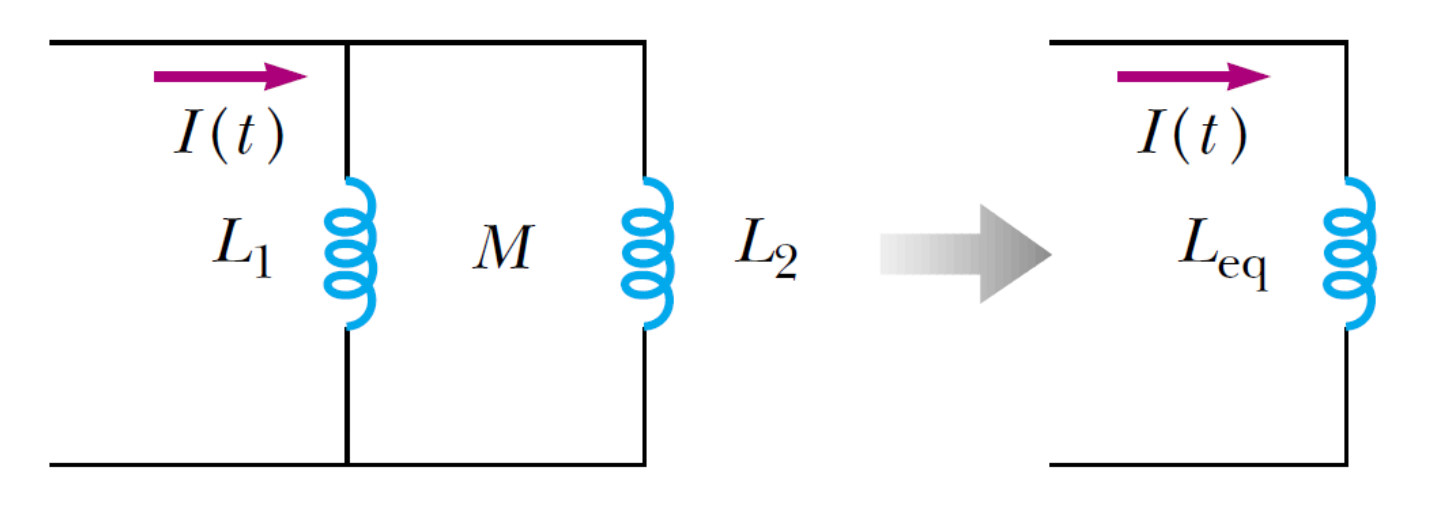
\includegraphics[scale = 0.3]{oz07/resources/Oz7Oef5.png}
\end{center}

\begin{description}[labelwidth=1.5cm, leftmargin=!]
    \item[Geg. :] $L_1$, $L_2$ en $M$
    \item[Gevr. :] $L_{eq}$ ? 
    \item[Opl. :]
        \begin{description}[labelwidth=1.5cm, leftmargin=!]
            \item[Gevr. :]  $L_{eq}$ ?
            \item[Opl. :]   
                Stel er is een spanningsbron $\mathcal{E}$. We krijgen de volgende spanningsvergelijkingen: 
                \begin{align}
                    \mathcal{E} 
                        &= - L_1 \frac{dI_1}{dt} - M \frac{dI_2}{dt} \tag{1} \\
                    \mathcal{E} 
                        &= - L_2 \frac{dI_2}{dt} - M \frac{dI_1}{dt} \tag{2} \\
                    \mathcal{E}
                        &= - L_{eq} \frac{dI}{dt}.  \tag{3}
                \end{align}
                met $I = I_1 + I_2$. Uit (1) vinden we
                \begin{equation*}
                    - \frac{dI_1}{dt} = \frac{\mathcal{E}}{L_1} + \frac{M}{L_1}\frac{dI_2}{dt}
                \end{equation*}
                wat we invullen in (2)
                \begin{equation*}
                    \mathcal{E} = - L_2 \frac{dI_2}{dt} + M \left(\frac{\mathcal{E}}{L_1} + \frac{M}{L_1}\frac{dI_2}{dt}\right) 
                \end{equation*}
                wat we herschrijven tot
                \begin{equation}
                    (-L_1L_2 + M^2)\frac{dI_2}{dt} = \mathcal{E}(L_1 - M) \tag{4}.
                \end{equation}
                Uit (2) vinden we
                \begin{equation*}
                    - \frac{dI_2}{dt} = \frac{\mathcal{E}}{L_2} + \frac{M}{L_2}\frac{dI_1}{dt}
                \end{equation*}
                wat we invullen in (1)
                \begin{equation*}
                    \mathcal{E} = - L_1 \frac{dI_1}{dt} + M \left(\frac{\mathcal{E}}{L_2} + \frac{M}{L_2}\frac{dI_1}{dt}\right)
                \end{equation*}
                wat we herschrijven tot
                \begin{equation}
                    (-L_1L_2 + M^2)\frac{dI_1}{dt} = \mathcal{E}(L_2 - M). \tag{5}
                \end{equation}
                Als we (4) en (5) optellen vinden we
                \begin{equation*}
                    (-L_1L_2 + M^2)\left(\frac{dI_1}{dt} + \frac{dI_2}{dt}\right) = \mathcal{E}(L_1 + L_2 - 2M)
                \end{equation*}
                sinds (3) geldt, volgt
                \begin{equation*}
                    L_{eq} = - \frac{-L_1L_2 + M^2}{L_1 + L_2 - 2M} = \frac{L_1L_2 - M^2}{L_1 + L_2 - 2M}
                \end{equation*}
        \end{description}
\end{description}

\vspace{1cm}